
% Copyright 2004 by Till Tantau <tantau@users.sourceforge.net>.
%
% In principle, this file can be redistributed and/or modified under
% the terms of the GNU Public License, version 2.
%
% However, this file is supposed to be a template to be modified
% for your own needs. For this reason, if you use this file as a
% template and not specifically distribute it as part of a another
% package/program, I grant the extra permission to freely copy and
% modify this file as you see fit and even to delete this copyright
% notice. 

\documentclass{beamer}
\usepackage{media9}
% Replace the \documentclass declaration above
% with the following two lines to typeset your 
% lecture notes as a handout:
%\documentclass{article}
%\usepackage{beamerarticle}
\usepackage{listings}
%\usepackage{graphicx}
\usepackage{wrapfig}
\usepackage{amsmath}
\usepackage{polski}
\usepackage[utf8]{inputenc}
\usepackage[polish]{babel}
%\usepackage[final]{graphicx}
\usepackage{subfig}
\usepackage{color}
\usepackage{amsmath}


\definecolor{mygreen}{rgb}{0,0.6,0}
\definecolor{mygray}{rgb}{0.5,0.5,0.5}
\definecolor{mymauve}{rgb}{0.58,0,0.82}

\lstset{ %
  backgroundcolor=\color{white},   % choose the background color; you must add \usepackage{color} or \usepackage{xcolor}; should come as last argument
  basicstyle=\footnotesize,        % the size of the fonts that are used for the code
  breakatwhitespace=false,         % sets if automatic breaks should only happen at whitespace
  breaklines=true,                 % sets automatic line breaking
  captionpos=b,                    % sets the caption-position to bottom
  commentstyle=\color{mygreen},    % comment style
  deletekeywords={...},            % if you want to delete keywords from the given language
  escapeinside={\%*}{*)},          % if you want to add LaTeX within your code
  extendedchars=true,              % lets you use non-ASCII characters; for 8-bits encodings only, does not work with UTF-8
  frame=single,	                   % adds a frame around the code
  keepspaces=true,                 % keeps spaces in text, useful for keeping indentation of code (possibly needs columns=flexible)
  keywordstyle=\color{blue},       % keyword style
  language=Java,                 % the language of the code
  morekeywords={*,...},            % if you want to add more keywords to the set
  numbers=left,                    % where to put the line-numbers; possible values are (none, left, right)
  numbersep=5pt,                   % how far the line-numbers are from the code
  numberstyle=\tiny\color{mygray}, % the style that is used for the line-numbers
  rulecolor=\color{black},         % if not set, the frame-color may be changed on line-breaks within not-black text (e.g. comments (green here))
  showspaces=false,                % show spaces everywhere adding particular underscores; it overrides 'showstringspaces'
  showstringspaces=false,          % underline spaces within strings only
  showtabs=false,                  % show tabs within strings adding particular underscores
  stepnumber=2,                    % the step between two line-numbers. If it's 1, each line will be numbered
  stringstyle=\color{mymauve},     % string literal style
  tabsize=2,	                   % sets default tabsize to 2 spaces
  title=\lstname                   % show the filename of files included with \lstinputlisting; also try caption instead of title
}
\usefonttheme{serif}

% There are many different themes available for Beamer. A comprehensive
% list with examples is given here:
% http://deic.uab.es/~iblanes/beamer_gallery/index_by_theme.html
% You can uncomment the themes below if you would like to use a different
% one:
%\usetheme{AnnArbor}
%\usetheme{Antibes}
%\usetheme{Bergen}
%\usetheme{Berkeley}
%\usetheme{Berlin}
%\usetheme{Boadilla}
%\usetheme{boxes}
%\usetheme{CambridgeUS}
%\usetheme{Copenhagen}
%\usetheme{Darmstadt}
%\usetheme{default}
%\usetheme{Frankfurt}
\usetheme[hideothersubsections]{Goettingen}
%\usetheme{Hannover}
%\usetheme{Ilmenau}
%\usetheme{JuanLesPins}
%\usetheme{Luebeck}
%\usetheme{Madrid}
%\usetheme{Malmoe}
%\usetheme{Marburg}
%\usetheme{Montpellier}
%\usetheme{PaloAlto}
%\usetheme{Pittsburgh}
%\usetheme{Rochester}
%\usetheme{Singapore}
%\usetheme{Szeged}
%\usetheme{Warsaw}

\title{Analiza zjawisk kaskadowych w sieciach transportowych}

% A subtitle is optional and this may be deleted
%\subtitle{Optional Subtitle}

\author[Tomasz Szypuła]{Tomasz Szypuła}

% - Give the names in the same order as the appear in the paper.
% - Use the \inst{?} command only if the authors have different
%   affiliation.

\institute[Politechnika Warszawska] % (optional, but mostly needed)
{
  %\inst{1}%
  Wydział Fizyki\\
  Politechnika Warszawska
 

% - Use the \inst command only if there are several affiliations.
% - Keep it simple, no one is interested in your street address.
}

%\date{Conference Name, 2013}
% - Either use conference name or its abbreviation.
% - Not really informative to the audience, more for people (including
%   yourself) who are reading the slides online

\subject{Theoretical Computer Science}
% This is only inserted into the PDF information catalog. Can be left
% out. 

% If you have a file called "university-logo-filename.xxx", where xxx
% is a graphic format that can be processed by latex or pdflatex,
% resp., then you can add a logo as follows:

% \pgfdeclareimage[height=0.5cm]{university-logo}{university-logo-filename}
% \logo{\pgfuseimage{university-logo}}

\usepackage{pgf}  
%\setbeamertemplate{navigation symbols}{\insertlogo}
%\pgfdeclareimage[height=1.3cm]{PW}{PW}
%\logo{\pgfuseimage{PW}}
\titlegraphic{
\includegraphics[scale=0.45,trim=10cm 0 0 1cm]{titlegraphic.png}}
\addtobeamertemplate{footline}{}{%
\makebox[\paperwidth]{%
    \hspace{0.04\textwidth}
    \hfill{}%
    \raisebox{2ex}[0pt][0pt]{
\includegraphics[width=0.8cm,keepaspectratio]{PW}}\hspace{0.04\textwidth}%
}%
}
% Delete this, if you do not want the table of contents to pop up at
% the beginning of each subsection:
\AtBeginSubsection[]
{
  \begin{frame}<beamer>{Plan}
    \tableofcontents[currentsection,currentsubsection]
  \end{frame}
}

% Let's get started
\begin{document}


\begin{frame}
  \titlepage
\end{frame}

\begin{frame}{Plan Prezentacji}
  \tableofcontents
  % You might wish to add the option [pausesections]
\end{frame}

% Section and subsections will appear in the presentation overview
% and table of contents.
\section{Wstęp}

\subsection{Cel Pracy}

\begin{frame}{Cel pracy}
Wyznaczyć 
\begin{enumerate}
\item Współczynnik Korelacji Pearson
\item Współczynnik Korelacji Spearmana (rangowa korelacja Pearsona)
\end{enumerate}
\pause
Dla sieci 
\begin{enumerate}
\item ARABIDOPSIS MULTIPLEX GPI
NETWORK
\item ARXIV NETSCIENCE MULTIPLEX
\item PADGETT-FLORENTINE-FAMILIES
MULTIPLEX NETWORK
\end{enumerate}
\end{frame}

\subsection{Dane}

\begin{frame}{ARABIDOPSIS MULTIPLEX GPI
NETWORK}
Opis \\
\vspace{5mm}
\textit{We consider different types of genetic interactions for organisms in the Biological General
Repository for Interaction Datasets (BioGRID, thebiogrid.org), a public database that
archives and disseminates genetic and protein interaction data from humans and model
organisms. BioGRID currently includes more than 720,000 interactions that have been
curated from both high-throughput data sets and individual focused studies using over
41,000 publications in the primary literature. We use BioGRID 3.2.108 (updated 1 Jan 2014).}
\end{frame}
\begin{frame}{ARABIDOPSIS MULTIPLEX GPI
NETWORK}
Poziomy 
\begin{enumerate}
\item Direct interaction
\item Physical association
\item Additive genetic interaction defined by inequality
\item Suppressive genetic interaction defined by inequality
\item Synthetic genetic interaction defined by inequality
\item Association
\item Colocalization
\end{enumerate}
\end{frame}

\begin{frame}{ARXIV NETSCIENCE MULTIPLEX}
Opis\\
\vspace{5mm}
\textit{The multiplex consists of layers corresponding to different arXiv categories. To restrict the
analysis to a well-defined topic of research, we only included papers with "networks" in the
title or abstract up to May 2014.}
\end{frame}
\begin{frame}{ARXIV NETSCIENCE MULTIPLEX}
Poziomy
\begin{enumerate}
\item physics.soc-ph
\item physics.data-an
\item physics.bio-ph
\item math-ph
\item math.OC
\item cond-mat.dis-nn
\item cond-mat.stat-mech
\item q-bio.MN
\item q-bio
\item q-bio.BM
\item nlin.AO
\item cs.SI
\item cs.CV
\end{enumerate}
\end{frame}

\begin{frame}{PADGETT-FLORENTINE-FAMILIES
MULTIPLEX NETWORK}
Opis\\
\vspace{5mm}
\textit{The multiplex social network consists of 2 layers (marriage alliances and business
relationships) describing florentine families in the Renaissance.}
\end{frame}
\begin{frame}{PADGETT-FLORENTINE-FAMILIES
MULTIPLEX NETWORK}
Poziomy
\begin{enumerate}
\item marriage alliances
\item business relationships
\end{enumerate}
\end{frame}
 
\subsection{Nowe pojęcia}
\begin{frame}{\textit{Property matrix \textbf{P}}}
Sieci wielopoziomowe zazwyczaj były reprezentowane przez macierze sąsiedztwa. Do liczenia miar podobieństwa jednak praktyczniejsza może okazać się macierz właściwości \textbf{P}. 
\pause
\begin{theorem}
i)  the columns correspond to a set \textbf{S} of network structures (nodes, edges, triangles, . . . )
\\(ii)  the rows correspond to a set \textbf{C} of contexts where these structures are observed (layers, groups,snapshots, . . . )
\\(iii)\textbf{P}$_{s,c}$ is the value of an observational function mapping each pair structure/context into a number(degree, distance, . . . ).
\end{theorem}
\begin{itemize}
\item<3> Dla mnie \textbf{C} czyli kontekst to warstwa
\item<4> Strukturą \textbf{S} będą węzły
\item<5> Funkcją mapującą będą stopnie węzłów
\end{itemize}
\end{frame}

\begin{frame}{Macierz \textbf{P}}
Przykładowa macierz \textbf{P} do reprezentacji stopni węzłów.
\center
\begin{tabular}{l|ccccc}
      & $n_1$ & $n_2$ & $n_3$ & $n_4$ & $n_5$ \\\hline
$l_1$ & 2     & 1     &     4 &   2   &  2   \\
$l_2$ &4    & 3     &     NA &   1   &  3   \\
\end{tabular}
\pause
Mając już każdą warstwą przedstawioną jako wektor, możemy policzyć korelacje Pearsona (i Spearmana) między różnymi wektorami.
\end{frame}
\section{Korelacja Pearsona i Spearmana}
\subsection{Pearson}
\begin{frame}{Korelacja Pearsona}
Korelacja Pearsona jest miarą liniowej Korelacji pomiędzy dwoma zmiennymi (wektorami) $\mathbb{X}$ i $\mathbb{Y}$. Przyjmuje wartości z zakresu $<-1,1>$
\pause
\begin{itemize}
\item[1] całkowita dodatnia korelacja
\item[-1] całkowita ujemna korelacja
\item[0] brak korelacji liniowej
\end{itemize}

\end{frame}
\begin{frame}{Korelacja Pearsona}
Współczynnik korelacji Pearsona został policzony wzorem
\begin{align*}
\textit{Pearson}=
\frac{[p_{l_1} - \textit{mean}(p_{l_1})]'[p_{l_2} - \textit{mean}(p_{l_2})]}{||[p_{l_1} - \textit{mean}(p_{l_1}]||||[p_{l_2} - \textit{mean}(p_{l_2})]||}
\end{align*}
Gdzie $p$ jest właśnie macierzą \textbf{P} wyżej omówioną.
\end{frame}
\subsection{Spearman}
\begin{frame}{Korelacja Spearmana}
Współczynnik korealcji Spearmana jest między dwoma zmiennymi $\mathbb{X}$ i $\mathbb{Y}$ jest równy korelacji Pearsona między wartościami rang tych dwóch zmiennych, $\rho(\mathbb{X})$ i $\rho(\mathbb{Y})$.
\\
\pause
Podczas gdy korelacja Pearsona bada liniowe zależności. Korelacja Spearmana bada monotoniczne zależności.
\pause
Intuicyjnie, współczynnik korelacji Spearmana będzie wysoki, gdy obserwacje mają podobną rangę w stosunku do wartości. 
\end{frame}

\section{Wyniki}
\subsection{Heatmapy}
\begin{frame}{Pearson, ARABIDOPSIS} 
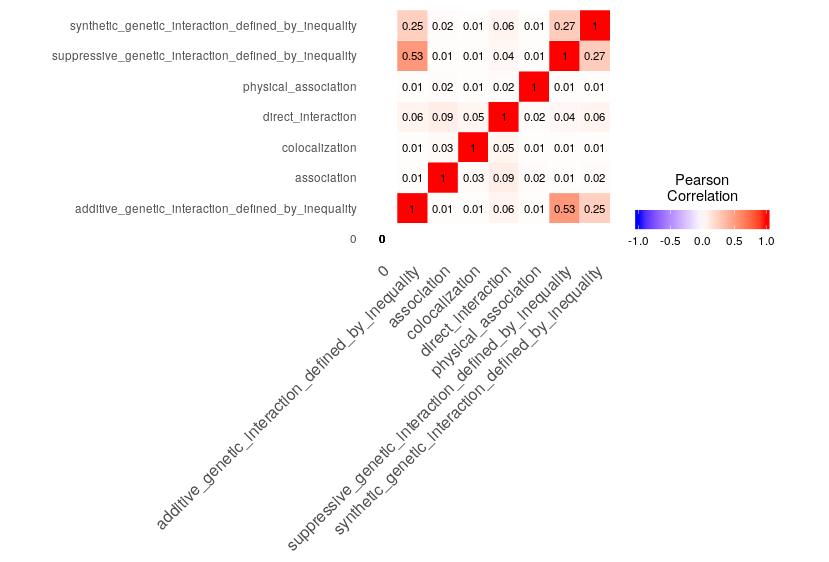
\includegraphics[scale=0.46]{heamapPearson1}
\end{frame}
\begin{frame}{Pearson, ARXIV} 
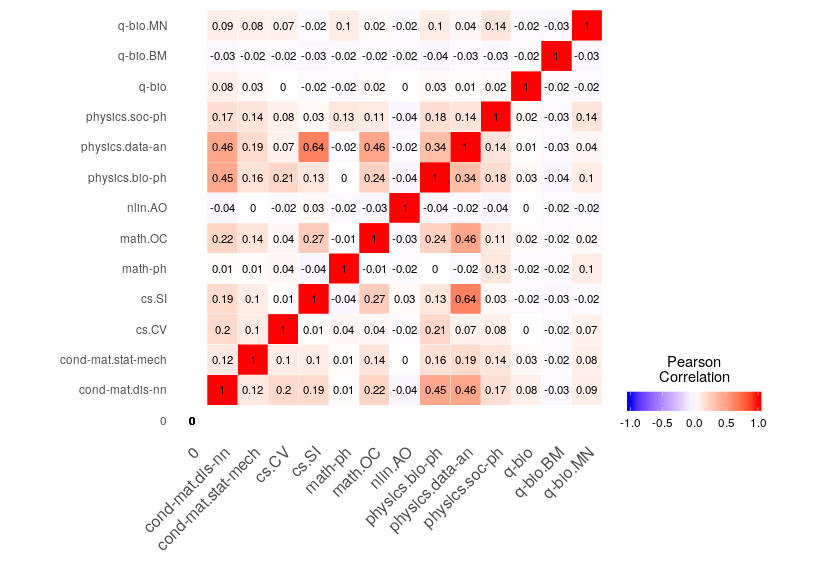
\includegraphics[scale=0.46]{heamapPearson2}
\end{frame}
\begin{frame}{Pearson, PADGETT-FLORENTINE-FAMILIES} 
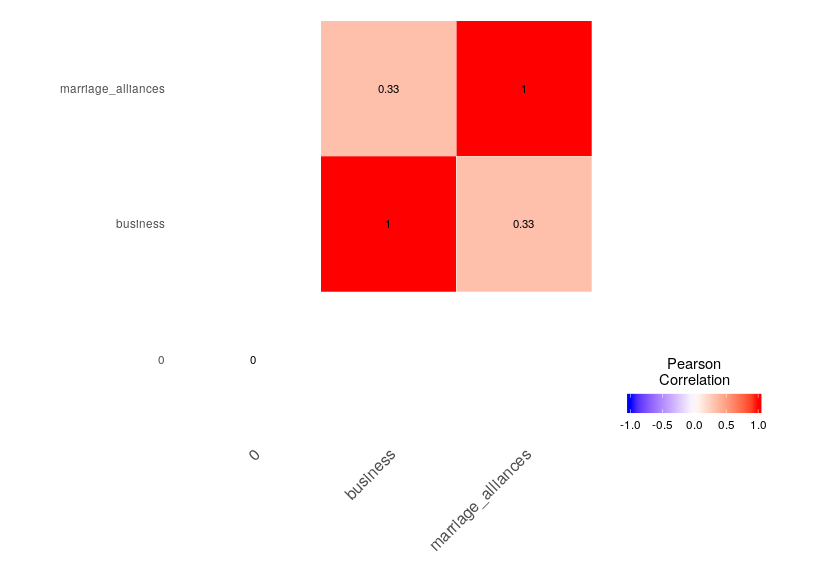
\includegraphics[scale=0.46]{heamapPearson3}
\end{frame}

\begin{frame}{Spearman, ARABIDOPSIS} 
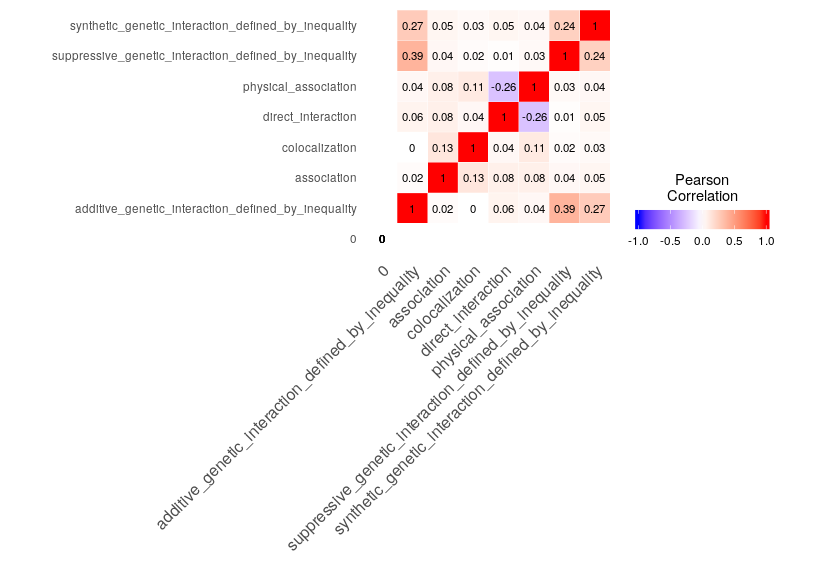
\includegraphics[scale=0.46]{heamapSpearman1}
\end{frame}
\begin{frame}{Spearman, ARXIV} 
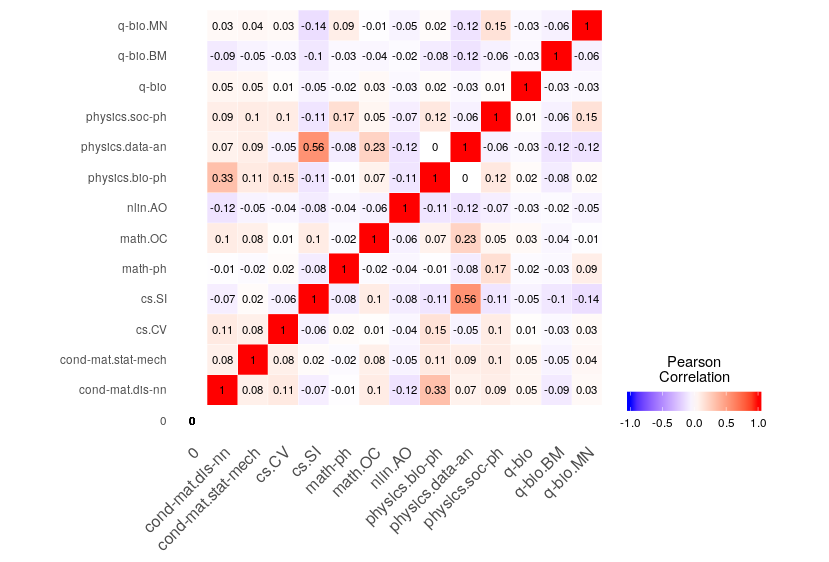
\includegraphics[scale=0.46]{heamapSpearman2}
\end{frame}
\begin{frame}{Spearman, PADGETT-FLORENTINE-FAMILIES} 
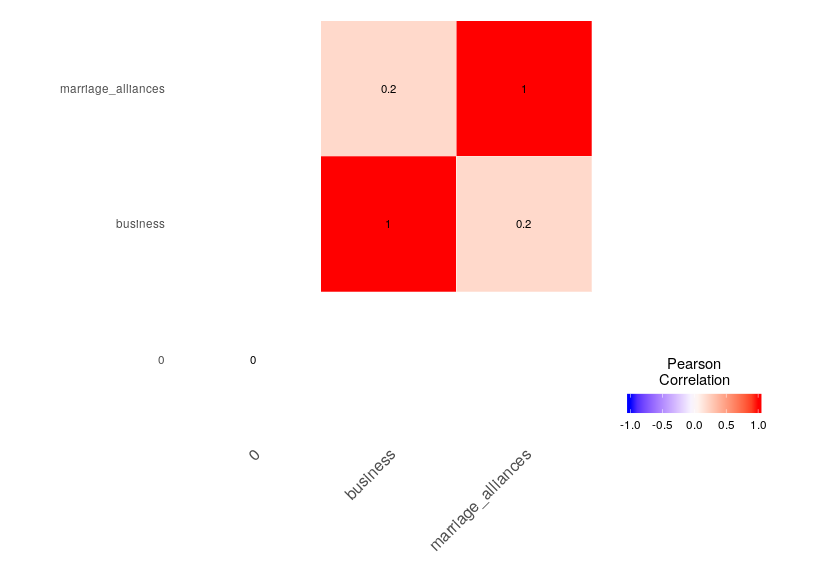
\includegraphics[scale=0.46]{heamapSpearman3}
\end{frame}

\subsection{Wykresy}
\begin{frame}{Pearson/Spearman, ARABIDOPSIS} 
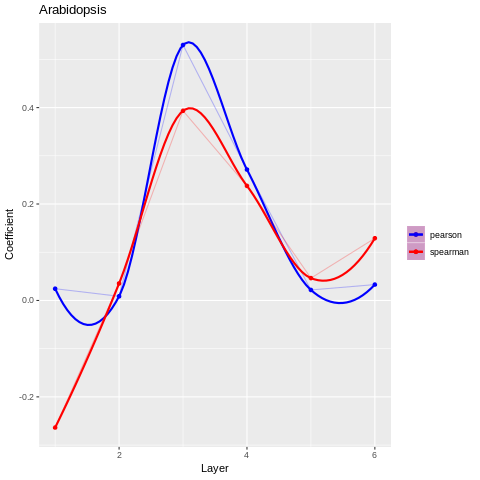
\includegraphics[scale=0.5]{plot1}
\end{frame}
\begin{frame}{Pearson/Spearman, ARXIV} 
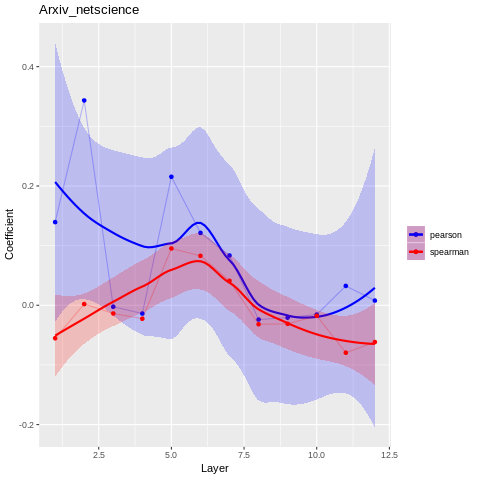
\includegraphics[scale=0.5]{plot2}
\end{frame}
\begin{frame}{Pearson/Spearman, PADGETT-FLORENTINE-FAMILIES} 
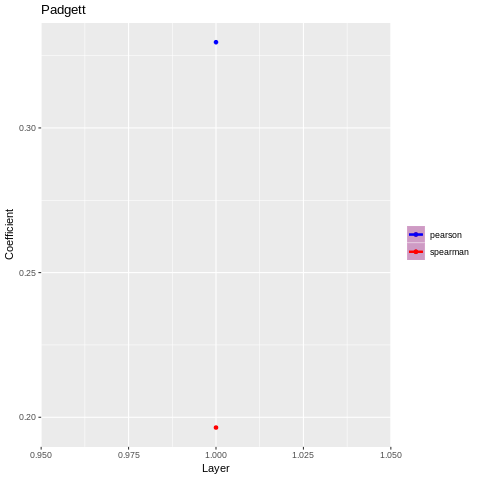
\includegraphics[scale=0.5]{plot3}
\end{frame}

\subsection{Boxploty}
\begin{frame}{Pearson} 
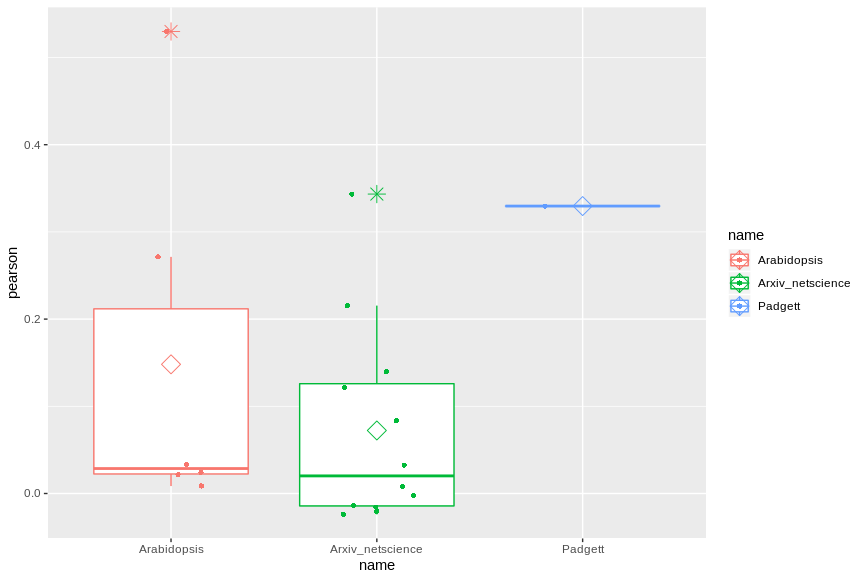
\includegraphics[scale=0.42]{boxplotPearson}
\end{frame}
\begin{frame}{Spearman} 
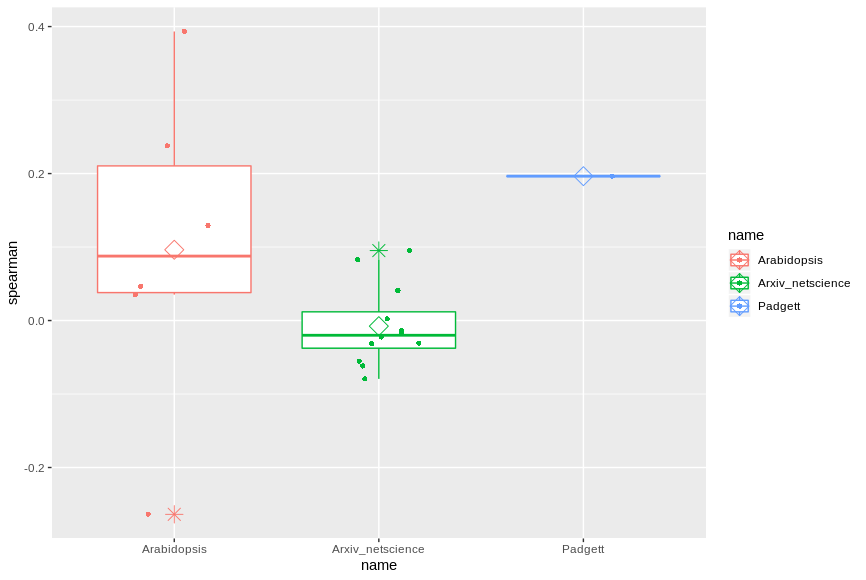
\includegraphics[scale=0.42]{boxplotSpearman}
\end{frame}
\end{document}


